
\section{Towards System 2 RAG in the wild}

% \subsubsection{Monolithic models to compound AI systems}

Towards productizing generative AI, there has been a shift from monolithic models to compound AI systems~\cite{kandogan2024blueprint} that incorporate various components other than LLMs for data retrieval, coordination, and utilizing proprietary models and services. Examples of such systems include Hiring Assistant by LinkedIn~\cite{linkedin-assistant}, AI-BI Genie by Databricks~\cite{databricks-aibi}, Agentforce by Salesforce~\cite{salesforce-agentforce}, and Magentic-One by Microsoft~\cite{microsoft-magentic}, among others. These systems are designed to ensure performance for complex tasks, adaptability to heterogeneous data and use cases, and a higher degree of trust in the production setting.

\stitle{Motivating example.}
Consider LinkedIn and Indeed, two global job-matching and hiring platforms in the HR domain. These companies are employing RAG-based workflows for a multitude of tasks in HR, such as matching, recruitment, and career guidance, among others~\cite{indeed-ai-blog, linkedin-ai-blog}. 
Given the task of matching job seekers with job postings, a popular use-case of generative AI is communicating meaningful explanations to job seekers about their relevance to the job. To support such a use-case, enterprises use RAG to infuse domain-specific relevant information, which guides the generation of explanations using LLMs~\cite{indeed-ai-blog}. Identifying the relevant information to be provided to the LLM in such a domain-specific context can be challenging due to the heterogeneity and scale of the data. Moreover, within such a production-oriented setting, enterprises have to remain cognizant of real-world constraints such as cost, latency, accuracy, and trustworthiness.


% \subsubsection{Data Heterogeneity}

\subsection{Data Heterogeneity in the Wild}
 Within an enterprise setting, different teams in an organization manage project-specific sources of data, collected and often transformed through various workflows over time. Such an observation is derived from the authors' experience working with enterprise data in the human resources (HR) domain at \company. 
For example, going back to the example of explaining job seeker and job posting match, a team tasked with such work will be interested in unstructured resumes and job descriptions, structured data extracted from the text and their representations, and HR domain-specific knowledge, \ie, relationships among different concepts such as jobs and benefits. Another team working on assisting job-seekers with search (\eg role and company) will be more interested in rather job market trends, company-specific information and search logs, among others. 

\begin{figure}[!htb] 
  \centering
  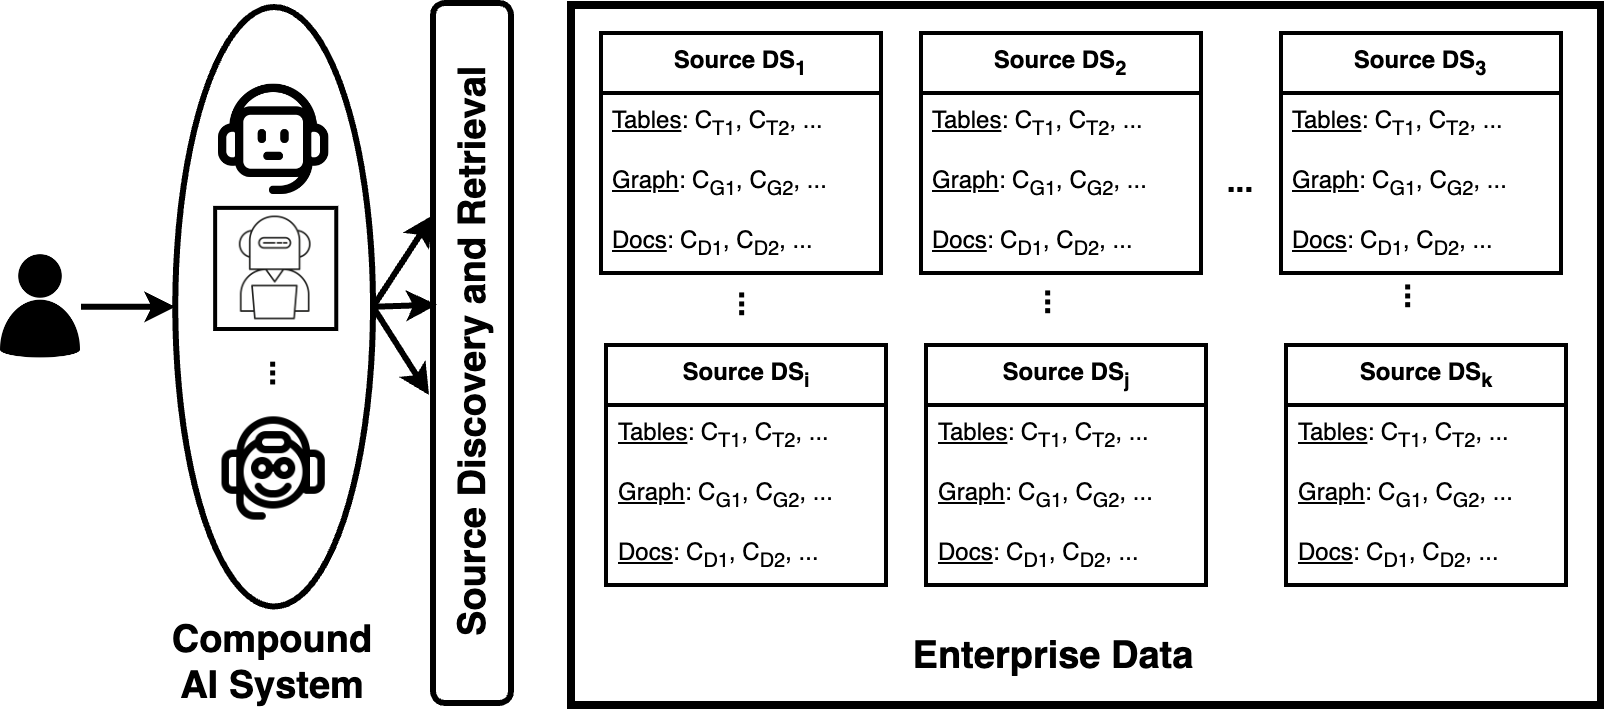
\includegraphics[width=0.65\linewidth]{submissions/Estevam2024/figures/mmd-lake.drawio.png}
  \caption{Conceptual data model for RAG in the wild.}
  \label{fig:cas_enterprise} 
\end{figure}

We introduce the data model for such a setting in Figure~\ref{fig:cas_enterprise}: \emph{compound AI systems} operating over such enterprise data~\cite{feng2024cmdbench}. The data model is multi-granular and multi-modal. Each team-specific data source $DS_i$ represents a collection of sources ($S_m \in DS_i$) corresponding to different modalities ($m$)  --- such as multiple tables and documents --- created by specific teams. While enterprises may contain data corresponding to other modalities such as audio, video, and image, we limit our scope to documents ($m=D$), tables ($m=T$), and graphs ($m=G$) in this case. Each data source is organized in a hierarchical manner --- at the coarse-grained level data is organized in data sources $DS_i$. Within each data source, data is organized in various collections $C_m$ depending on the modality. Within each collection, data can be stored and managed by different systems ($C_{mi}$) depending on the downstream application such as data warehouse, data lake, and lakehouse systems~\cite{DBLP:journals/bdcc/NambiarM22,armbrust2021lakehouse}. Therefore, the assumption of traditional RAG where these data sources or collections or databases are known beforehand, breaks down in such a setting. Rather a multi-step approach to data discovery (closer to System 2) is required to identify the relevant coarse- and fine-grained data given a user query.

%\subsection{System considerations}
%\begin{figure}[!htb] 
%  %\vspace{-10pt}
%  \centering
%  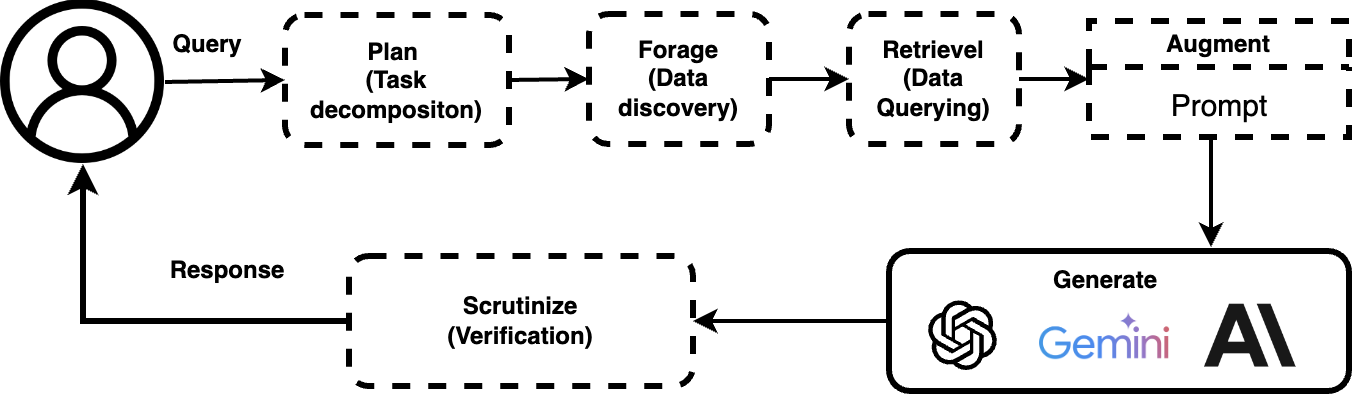
\includegraphics[width=0.8\linewidth]{submissions/Estevam2024/figures/cas-rag.drawio.png}
%  \caption{``System 2'' approach to RAG on enterprise infrastructure through agentic $workflows}
%  \label{fig:sys-rag} 
%  %\vspace{-15pt}
% \end{figure}

\subsection{Rethinking RAG}
To this end, a major consideration in moving a RAG pipeline from System 1 to System 2 thinking involves shifting toward deliberate analytics and explicit reasoning.
This transition means that decisions—such as when and where to retrieve information, how much data to retrieve, and how to integrate retrieved information into the generated response—should be made through rigorous reasoning. This reasoning should carefully assess the unique characteristics of the task, data, tools, and available models to ensure outcomes that are both optimal and context-aware. Note that recently released LLM such as \emph{o1}\footnote{https://openai.com/o1/} instruments slow thinking by executing some type of reasoning mechanism before generating the final answer. Even though there has been discussions within certain research circles, which mentions the possibility of having chain of thought and self-reflection empowering \emph{o1} models before they generate an answer, it is important to state that no official documentation confirms the use of such techniques in the \emph{o1} models) ---- One consequence of this new reasoning capabilities of these models is the additional time spent thinking, that makes it more effective for complex reasoning tasks, particularly in science and mathematics. 
However, the additional step leads to higher latency during inference, which may vary depending on the task. In addition to that, \emph{o1} is similar to the earlier monolithic LLMs where the parametric knowledge remains abstract, thereby lacking transparency and controllability as no affordances are provided to the users to interact with the decision-making process.

 
Given a knowledge-intensive task that requires complex reasoning and planning, a systematic approach is necessitated to ensure transparency of the workflow, integrate user guidance at various steps, and enable optimization under real-world constraints such as cost, latency, and accuracy. As illustrated in Figure~\ref{fig:sys-rag2}, at the core of the System 2 RAG pipeline lies a planner, which functions as a reasoning module. 
This planner is grounded in specific tasks and budgets (\eg time, cost, quality) and operates by foraging and analyzing the properties of data and agents within the registries. Moreover, retrieval is expanded to not only extracting information from documents but also other formats of raw data and data management systems as outlined in Figure~\ref{fig:cas_enterprise}. Adaptation of retrieval to large-scale heterogenous data necessitates reconciliation and reranking of retrieved information. With the presence of heterogeneous information, the augmented generation requires further scrutinization through fact-checking and verification,
